\documentclass{article}

\usepackage{calculator}
\usepackage{calculus}

\usepackage{fancyhdr}
\usepackage{extramarks}
\usepackage{amsmath}
\usepackage{amsthm}
\usepackage{amsfonts}
\usepackage{tikz}
\usepackage[plain]{algorithm}
\usepackage{algpseudocode}
\usepackage{tikz,pgfplots,multicol}
\usepackage[font=small,labelformat=empty]{caption}
\usetikzlibrary{automata,positioning,arrows,patterns}
\usepackage{enumitem}


\usepgfplotslibrary{fillbetween}


\newcommand{\boundellipse}[3]% center, xdim, ydim
{(#1) ellipse (#2 and #3)
}
%
% Basic Document Settings
%

\topmargin=-0.45in
\evensidemargin=0in
\oddsidemargin=0in
\textwidth=6.5in
\textheight=9.0in
\headsep=0.25in

\linespread{1.1}

\pagestyle{fancy}
\lhead{\hmwkAuthorName}
\chead{\hmwkClass\ (\hmwkClassInstructor\ \hmwkClassTime)}
\rhead{\hmwkTitle}
\lfoot{\lastxmark}
\cfoot{\thepage}

\renewcommand\headrulewidth{0.4pt}
\renewcommand\footrulewidth{0.4pt}

\setlength\parindent{0pt}

\setcounter{secnumdepth}{0}
\newcounter{partCounter}
\newcounter{homeworkProblemCounter}
\setcounter{homeworkProblemCounter}{1}
\nobreak\extramarks{Problem \arabic{homeworkProblemCounter}}{}\nobreak{}



%
% Homework Problem Environment
%
% This environment takes an optional argument. When given, it will adjust the
% problem counter. This is useful for when the problems given for your
% assignment aren't sequential. See the last 3 problems of this template for an
% example.
%
\newenvironment{homeworkProblem}[1][-1]{
    \ifnum#1>0
        \setcounter{homeworkProblemCounter}{#1}
    \fi
    \section{Problem \arabic{homeworkProblemCounter}}
    \setcounter{partCounter}{1}
    \enterProblemHeader{homeworkProblemCounter}
}{
    \exitProblemHeader{homeworkProblemCounter}
}

%
% Homework Details
%   - Title
%   - Due date
%   - Class
%   - Section/Time
%   - Instructor
%   - Author
%

\newcommand{\hmwkTitle}{HW \#15}
\newcommand{\hmwkDueDate}{May 4, 2017}
\newcommand{\hmwkClass}{MATH 1300}
\newcommand{\hmwkClassTime}{Section 005}
\newcommand{\hmwkClassInstructor}{Professor Braden Balentine}
\newcommand{\hmwkAuthorName}{\textbf{John Keller}}

%
% Title Page
%

\title{
    \vspace{2in}
    \textmd{\textbf{\hmwkClass:\ \hmwkTitle}}\\
    \normalsize\vspace{0.1in}\small{Due\ on\ \hmwkDueDate\ at 10:00am}\\
    \vspace{0.1in}\large{\textit{\hmwkClassInstructor\ \hmwkClassTime}}
    \vspace{3in}
}

\author{\hmwkAuthorName}
\date{}

\renewcommand{\part}[1]{\textbf{\large Part \Alph{partCounter}}\stepcounter{partCounter}\\}

%
% Various Helper Commands
%

% Useful for algorithms
\newcommand{\alg}[1]{\textsc{\bfseries \footnotesize #1}}

% For derivatives
\newcommand{\deriv}[1]{\frac{\mathrm{d}}{\mathrm{d}x} (#1)}

% For partial derivatives
\newcommand{\pderiv}[2]{\frac{\partial}{\partial #1} (#2)}

% Integral dx
\newcommand{\dx}{\mathrm{d}x}

% Alias for the Solution section header
\newcommand{\solution}{\textbf{\large Solution}}

% Probability commands: Expectation, Variance, Covariance, Bias
\newcommand{\E}{\mathrm{E}}
\newcommand{\Var}{\mathrm{Var}}
\newcommand{\Cov}{\mathrm{Cov}}
\newcommand{\Bias}{\mathrm{Bias}}


\usepackage{xcolor}
    \colorlet{Curve}{red!75!black}
    \colorlet{Tangent}{blue!75!black}
\usepackage{pgfplots}
    \pgfplotsset{compat=1.10}
    \usetikzlibrary{
        calc,
        intersections,
        math,
    }
    \makeatletter
        \def\parsenode[#1]#2\pgf@nil{%
            \tikzset{label node/.style={#1}}
            \def\nodetext{#2}
        }
        \tikzset{
            % define style for the points
            Point/.style={
                shape=circle,
                inner sep=0pt,
                minimum size=3pt,
            },
            add node at x/.style 2 args={
                name path global=plot line,
                /pgfplots/execute at end plot visualization/.append={
                        \begingroup
                        \@ifnextchar[{\parsenode}{\parsenode[]}#2\pgf@nil
                    \path [name path global = position line #1-1]
                        ({axis cs:#1,0}|-{rel axis cs:0,0}) --
                        ({axis cs:#1,0}|-{rel axis cs:0,1});
                    \path [xshift=1pt, name path global = position line #1-2]
                        ({axis cs:#1,0}|-{rel axis cs:0,0}) --
                        ({axis cs:#1,0}|-{rel axis cs:0,1});
                    \path [
                        name intersections={
                            of={plot line and position line #1-1},
                            name=left intersection
                        },
                        name intersections={
                            of={plot line and position line #1-2},
                            name=right intersection
                        },
                        label node/.append style={pos=1}
                    ] (left intersection-1) -- (right intersection-1)
                        node [label node]{\nodetext};
                    % ---------------------------------------------------------
                    % draw the tangent line from a bit right of the point on
                    % the curve to the intersection with the ordinate
                    % and draw the corresponding points
                    \draw [dashed] let
                        \p1=($ (left intersection-1) - (right intersection-1) $),
                        \p2=($ (left intersection-1)!sign(#1)*10mm!(right intersection-1) $),
                        %\p2=($ (left intersection+1) - (right intersection+1) $),
                        \p3=($ ({axis cs:0,0}) - (\p2) $),
                        \n1={\x3/\x1}	% slope of tangent line
                    in
                        (\p2) -- +($ {\n1}*(\x1,\y1) $)
	                        
%                        		node[right,node font=\scriptsize,gray] {$y=$\y1/\x1*sign(#1) $x+$}
%                            node [Point,fill=Tangent] (origin intersection) {}
                            node [Point,fill=Curve] at (left intersection-1) {}
                    ;
                    % ----------
                    % draw the horizontal line at the curve intersection point
                    % plus the label above/below the line
%                    \tikzmath{
%                        coordinate \c1;
%                        \c1=(left intersection-1) - (right intersection-1);
%                        \slope=\cy1/\cx1*sign(#1);
%                        \plusoffset = (#1+1);
%                    }
%                    \pgfmathsetmacro{\AboveBelow}{ \slope>0 ? "above" : "below" }
%                    \draw [dashed]
%                        ([xshift=sign(#1)*2.5mm] left intersection-1) --
%                        (left intersection-1) --
%                            node [\AboveBelow,node font=\scriptsize] {$y=\slope x+\plusoffset$}
%                        (left intersection-1 -| origin intersection) --
%                        +($ sign(#1)*(-2.5mm,0) $)
%                            coordinate [pos=0.5] (a)
%                    ;
%                    % draw the horizontal line at the ordinate intersection point
%                    \draw [dotted] (origin intersection)
%                        +($ sign(#1)*(-2.5mm,0) $) --
%                        (origin intersection);
%                    % draw vertical line left/right of the ordinate
%                    \pgfmathsetmacro{\LeftRight}{ #1<0 ? "right" : "left" }
%                    \draw [stealth-stealth] (origin intersection)
%                        +($ sign(#1)*(-1.25mm,0) $) -- (a)
%                            node [midway,\LeftRight,node font=\scriptsize] {$p$}
%                    ;
%                    % ---------------------------------------------------------
                        \endgroup
                },
            },
        }
    \makeatother
\makeatletter
\def\mathcolor#1#{\@mathcolor{#1}}
\def\@mathcolor#1#2#3{%
  \protect\leavevmode
  \begingroup
    \color#1{#2}#3%
  \endgroup
}
\makeatother
\begin{document}

\maketitle

\pagebreak

\section{Section 5.4}
\begin{enumerate}
\setcounter{enumi}{5}
	\item Sketch the area represented by $g(x)$. Then find $g'(x)$ in two ways: (a) by using the Part 1 of the Fundamental Theorem and (b) by evaluating the integral using Part 2 and then differentiating. $$g(x)=\int_{0}^{x}(1+\sqrt{t})dt$$
	\begin{center}
		\begin{tikzpicture} 
		    \begin{axis}[enlargelimits=0.1,axis lines=middle,ticks=none,ymin=-0.25,xmin=-0.5,xmax=10.5]
		    \addplot[samples=200,name path=f,domain=-0:10,blue] {1+x^0.5};
		
		    \path[name path=axis] (axis cs:0,0) -- (axis cs:10,0);
		
		    \addplot [
		        thick,
		        color=blue,
		        fill=blue, 
		        fill opacity=0.05
		    ]
		    fill between[
		        of=f and axis,
		        soft clip={domain=0:10},
		    ];
%		 Draw labels for the lines
		    \node [rotate=0] at (axis cs:  0,  -0.15) {$0$};
		    \node [rotate=0] at (axis cs:  10,  -0.15) {$x$};
		    \end{axis}
		\end{tikzpicture}  
	\end{center}
	\begin{enumerate}
		\item $$\begin{align}
		g(x)&=- \int_{0}^{x}(1+\sqrt{t}) dt\\
		&=- \int_{x}^{0}(1+\sqrt{t})dt\\
		g'(x)&=-1\cdot\frac{d}{dt}\left[\int_{0}^{x}(1+\sqrt{t}) dt\right]\\
		g'(x)&=\boxed{\frac{2x^\frac{2}{3}}{3}+x}
	\end{align}$$
		\item $$\begin{align}
			g(x)&=\int_0^x\left(1+\sqrt{t}\right)dt\\
			&=\left(t+\frac{2t^\frac{3}{2}}{3}\right)\Bigg]^x_0\\
			&=\left(x+\frac{2(x)^\frac{3}{2}}{3}\right)-\left(0+\frac{2(0)^\frac{3}{2}}{3}\right)\\
			&=\boxed{\frac{2x^\frac{2}{3}}{3}+x}
		\end{align}$$
	\end{enumerate}
\pagebreak
\setcounter{enumi}{17}
	\item Use Part 1 of the Fundamental Theorem of Calculus to find the derivative of the function. $$y=\int_{\sin x}^{\cos x}(1+v^2)^{10} dv$$\newline
	$$\begin{align}
		y&=- \int_{\cos x}^{\sin x}(1+v^2)^{10} dv\\
		&=- \int_{\cos x}^{\sin x}1+v^{20} dv\\
		\frac{d}{dy}(y)&=-1\cdot\frac{d}{dy}\left[\int_{\cos x}^{\sin x}1+v^{20} dv\right]\\
		y'&=-1\cdot \left(1+y^{20}\right)\\
		&=\boxed{-1-y^{20}}
	\end{align}$$
\setcounter{enumi}{22}
	\item On what interval is the curve $$y=\int_{0}^{x}\frac{t^2}{t^2+t+2}dt$$\
	$$\begin{align}
		= t-\frac{3\arctan \left(\frac{2\left(t+\frac{1}{2}}{\sqrt{7}}\right)}{\sqrt{7}}-\frac{1}{2}\ln\left|\left(1+\frac{1}{2}\right)^2+\frac{7}{4}\right|+C\\
		=x+\frac{1}{14}\left(-7\ln\left(x^2+x+2\right)-6\sqrt{7}\arctan\left(\frac{2x+1}{\sqrt{7}}\right)+\ln(128)+6\sqrt{7}\text{arccot}\left(\sqrt{7}\right)\right)
	\end{align}$$
\setcounter{enumi}{29}
	\item Let $$f(x)=
		\begin{cases}
	        0 & \text{if $x<0$} \\
		    x & \text{if $0\leq x \leq 1$} \\
			2-x & \text{if $1< x < 2$}\\
			0 & \text{if $x>2$}
  \end{cases}$$
  and
  $$g(x)=\int_{0}^{x}f(t)dt$$
  \begin{enumerate}
  	\item Find an expression for $g(x)$ similar to the one for $f(x)$.
  	\vspace{3cm}\pagebreak
  	\item Sketch the graphs of $f$ and $g$.
  	\begin{center}
		\pgfplotsset{width=13cm,height=5cm}
				\begin{tikzpicture}
				\begin{axis}[axis lines=middle]
					\addplot[dashed,domain=-2:0] {0};
					\addplot[dashed,domain=0:1] {x};
					\addplot[dashed,domain=1:2] {2-x};
					\addplot[dashed,domain=2:4] {0};
				\end{axis}
			\end{tikzpicture}
	\end{center}
  	\item Where is $f$ differentiable? Where is $g$ differentiable?
  	\vspace{2cm}
  \end{enumerate}
\end{enumerate}

\section{Section 5.5}
\begin{enumerate}
\setcounter{enumi}{14}
	\item Evaluate the indefinite integral. $$\int \frac{dx}{5-3x}$$\ 
	$$\begin{align}
		\int \frac{1}{5-3x}dx\\
		\int -\frac{1}{3u}du\\
		-\frac{1}{3}\cdot \int \frac{1}{u}du\\
		-\frac{1}{3}\ln|u|
		-\frac{1}{3}\ln|5-3x|\\
		-\frac{1}{3}\ln|5-3x|+C
	\end{align}$$
\setcounter{enumi}{67}
	\item If $f$ is continuous and $\int_{0}^{9}f(x)dx=4$, find $\int_{0}^{3}xf(x^2)dx$.
	\vspace{3cm}
\setcounter{enumi}{69}
	\item If $f$ is continuous on $\mathbb{R}$, prove that $$\int_{a}^{b}f(x+c)dx=\int_{a+c}^{b+c}f(x)dx$$
	$$\begin{align}
		\int_{a}^{b}f(x)dx+\int_{a}^{b}f(c)dx
	\end{align}$$
\end{enumerate}

\section{Section 6.1}
\begin{enumerate}
\setcounter{enumi}{1}
	\item Find the area of the shaded region.
	\begin{center}
		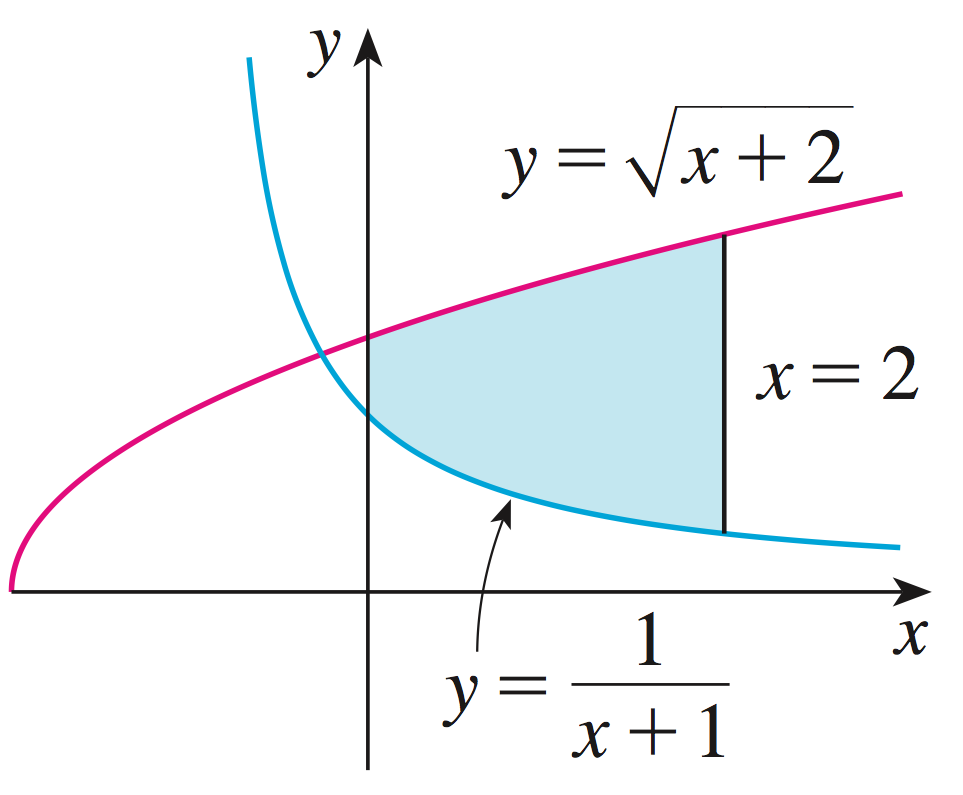
\includegraphics[width=4cm]{images/61pr2}
	\end{center}
	$$\begin{align}
		\int_{0}^{2}\left(-\frac{1}{1+x}+\sqrt{2+x}\right)dx = \frac{1}{3}\left(16-4\sqrt{2}\right)-\ln(3)\approx 2.3491
	\end{align}$$
\setcounter{enumi}{3}
	\item Find the area of the shaded region.
	\begin{center}
		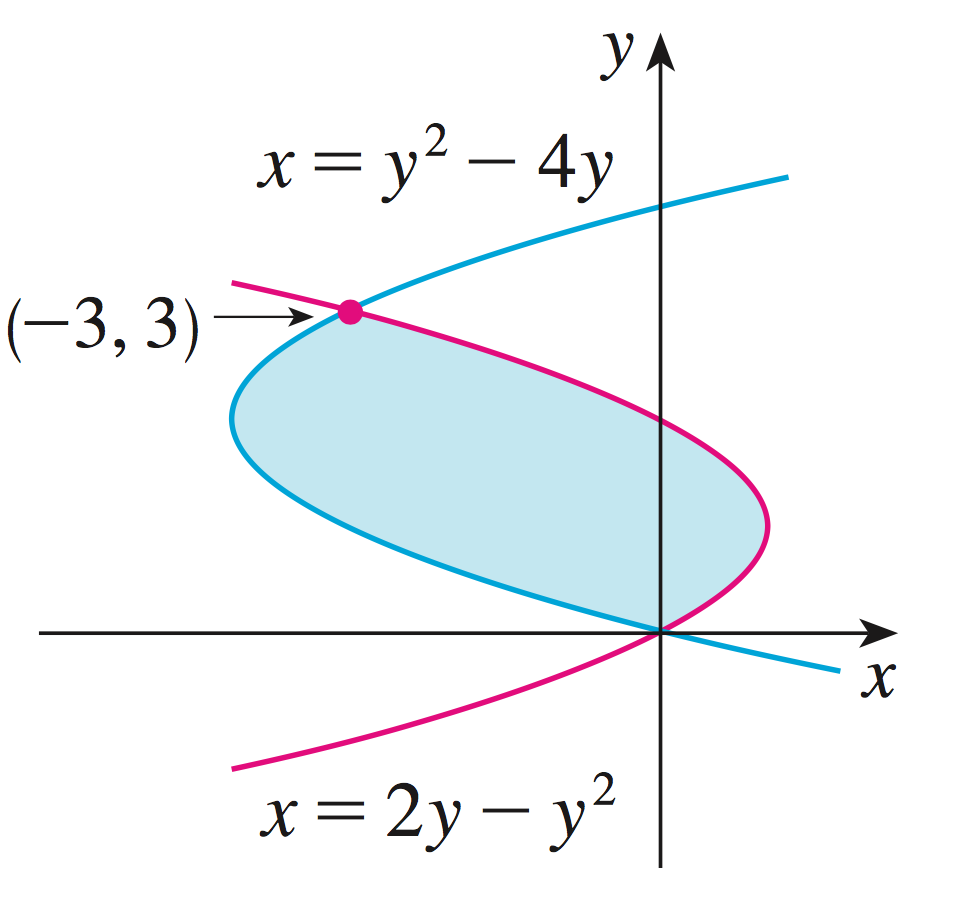
\includegraphics[width=4cm]{images/61pr4}
	\end{center}
	$$\begin{align}
		\int_{0}^{3}\left(y^2-4y\right)-\left(2y-y^2\right)\\
		\int_{0}^{3}2y^2-6y = \frac{2y^3}{3}-\frac{6y^2}{2}\Bigg]^3_0 = \left(\frac{2(3)^3}{3}-\frac{6(3)^2}{2}\right)-\left(\frac{2(0)^3}{3}-\frac{6(0)^2}{2}\right)=\boxed{-9}
	\end{align}$$
\setcounter{enumi}{9}
	\item Sketch the region enclosed by the given circles. Decide whether to integrate with respect to x or y. Draw a typical approximating rectangle and label its height and width. Then find the area of the region. $$4x+y^2=12,\qquad x=y$$
	\begin{center}
		\pgfplotsset{width=12cm,height=8cm,ymin=-7,xmin=-7,xmax=4}
				\begin{tikzpicture}
				\begin{axis}[axis lines=middle]
					\addplot[name path=fun1,samples=2,domain=-6.5:4]{x};
					\addplot[name path=fun2,samples=200,domain=-6.5:2.9999]{(12-4*x)^(0.5)};
					\addplot[name path=fun3,samples=200,domain=-6.5:2.9999]{-(12-4*x)^(0.5)};
					\node[label={90:{(2,2)}},circle,fill,inner sep=1pt] at (axis cs:2,2) {};
					\node[label={92:{(-6,-6)}},circle,fill,inner sep=1pt] at (axis cs:-6,-6) {};
				\end{axis}
			\end{tikzpicture}
	\end{center}
\end{enumerate}

\end{document}